\documentclass[12pt]{article}

\usepackage{sbc-template}

\usepackage{graphicx,url}

%\usepackage[brazil]{babel}   
\usepackage[utf8]{inputenc}  

\usepackage{makecell}
     
\sloppy

\title{Análise de Sentimentos utilizando Dicionários Léxicos\\ Uma Revisão Sistemática}

\author{Airton Bordin Junior\inst{1}}


\address{Instituto de Informática -- Universidade Federal de Goiás
  (UFG)\\
  Caixa Postal 131 -- 74690-900 -- Goiânia -- GO -- Brazil
}

\begin{document} 

\maketitle

\begin{abstract}
The increase in the number of Internet users in recent years has resulted in a growing content production by its users. Often, the WEB is used as a platform for debates, opinions, evaluations, etc. This fact, in line with the ease of obtaining the information, made the area of Sentiment Analysis, also called Opinion Mining, a growing interest on the part of reserachers.

One of the most used strategies in the process of Sentiment Analysis is the Lexical Dictionaries - a set of words and their polarities, generally defined as positive, negative or neutral. Although widely used, this approach has some challenges to overcome, such as identifying the domain of the text, for example - a word can have a completely different meaning depending on the context in which it is found.

The present work presents a Systematic Review of the literature to identify the main strategies adopted in the automatic creation and expansion of Lexical Dictionaries.
\end{abstract}

\begin{resumo} 
O aumento no número de usuários de Internet nos últimos anos teve como consequência uma crescentre produção de conteúdo por seus usuários. Frequentemente, a WEB é utilizada como plataforma para debates, opiniões, avaliações, etc. Esse fato, alinhado a facilidade de obtenção dessas informações, fez com que a área de Análise de Sentimentos, também chamada de Mineração de Opiniões, tivesse um interesse crescente por parte de pesquisadores. 

Uma das estratégias mais utilizadas no processo de Análise de Sentimentos é a utilização de Dicionários Léxicos  - conjunto de palavras e suas polaridades, geralmente definidas como positiva, negativa ou neutra. Apesar de amplamente utilizada, essa abordagem possui alguns desafios a serem superados, como a identificação do domínio do texto, por exemplo - uma palavra pode ter um significado completamente diferente, dependendo do contexto em que se encontra.

O presente trabalho apresenta uma Revisão Sistemática da literatura para identificar as principais estratégias adotadas na criação e expansão automatizada de Dicionários Léxicos.
\end{resumo}


\section{Introdução}
A Mineração de Opiniões, também chamada de Análise de Opiniões ou Análise de Sentimentos, é uma linha de pesquisa abrangente e que vem sendo tema de diversos trabalhos nos últimos anos. Como observado em \cite{liu2010multifaceted}, esse crescente interesse sobre o assunto ocorre principalmente devido ao aumento no número de usuários de Internet e o consequente crescimento da produção de conteúdo independente na rede, como opiniões, avaliações, entre outros. 

Essa área de estudo tem como principal desafio a Análise de Opiniões, descritas em linguagem natural, para a identificação da polaridade implícita ou explícita no texto. Essa polaridade é, na maior parte das vezes, identificada como uma escala de pontuação de sua característica positiva, negativa ou neutra.

Uma das principais técnicas para aumentar a acurácia a Análise de Sentimentos é a utilização de Dicionários de Dados. Esses dicionários contêm palavras previamente avaliadas por especialistas humanos, principalmente quanto à sua polaridade. Neste contexto, esse conjunto de palavras, juntamente com suas polaridades, é chamado de Dicionário Léxico ou Dicionário de Sentimentos. 

Porém, é evidente a limitação inerente à estratégia de utilização do Dicionário Léxico - a própria lista de palavras disponíveis. Esse fato muitas vezes limita a realização de uma análise mais profunda sobre determinado contexto. Nesse sentido, um dos principais desafios na área de Mineração de Opiniões é a criação e ampliação do Dicionário Léxico de forma automatizada, tema central do presente trabalho. Grande parte desses dicionários são construídos de forma manual, fato que caracteriza uma limitação óbvia para a maior parte dos contextos e domínios, como observado em \cite{duwairi2015detecting}. 

Existem, basicamente, 3 formas de criação e expansão de um Dicionário Léxico: manual -  processo realizado por especialistas humanos que analisam cada palavra, atribuindo uma Orientação Semântica para cada uma delas -  e duas formas (semi) automatizadas: baseada em Dicionário e baseada em Corpus. Frequentemente, essas técnicas são utilizadas em conjunto, principalmente a validação manual de Dicionários criados de forma automatizada. Criações de Dicionários utilizando somente abordagem manual, por sua característica limitante, são menos utilizadas e não serão abordadas de forma mais aprofundada no decorrer deste trabalho.

Consciente do problema de criação e expansão de Dicionários Léxicos para a Análise de Sentimentos, a ideia principal do presente trabalho é a realização de uma Revisão Sistemática da Literatura, conforme apresentada em \cite{Kitchenham2004}, de forma a identificar e analisar os principais trabalhos disponíveis sobre o tema. Esses trabalhos apoiarão na resolução das questões de pesquisa, apresentadas em detalhes na próxima seção. A análise dos artigos também auxiliará na identificação dos \emph{gaps} de pesquisa, que poderão ser explorados em trabalhos futuros.

\section{Estratégia da Revisão Sistemática}
A Revisão Sistemática da Literatura fornece uma forma estruturada, objetiva e reprodutível de identificar, avaliar e interpretar trabalhos relevantes em uma determinada área de conhecimento. A análise desses trabalhos apoia a resoluções das questões de pesquisa, que devem ser respondidas pelo projeto \cite{Kitchenham2004}.

A definição das questões da pesquisa é uma parte crítica da Revisão Sistemática. Essas mesmas questões são utilizadas de forma a orientar a estratégia de busca e palavras-chave dos artigos nas bases de dados escolhidas.

As questões norteiam, também, os dados e informações que serão relevantes e extraídos dos trabalhos selecionados. Para este trabalho, as questões de pesquisa são as seguintes:

\label{sec:questoesPesquisa}
\begin{itemize}
	\item{Quais as principais estratégias utilizadas para a classificação de sentimentos?}
	\item{Quais as principais técnicas empregadas na criação e expansão de Dicionários Léxicos?}
	\item{Como a diferença de contexto e domínio vem sendo tratada no contexto de Análise de Sentimentos?}
	\item{Que métricas estão sendo utilizadas para avaliar a qualidade dos algoritmos de criação e expansão de Dicionários Léxicos?}
\end{itemize}

Para a elaboração desta Revisão Sistemática, foram realizadas buscas nas seguintes bases de dados: \emph{Science Direct}, \emph{IEEEXplore}, \emph{ACM Digital Library}, \emph{Research Gate}, \emph{Semantic Scholar}. Essas buscas tem por objetivo coletar os trabalhos primários sobre o tema proposto para a identificação do estado obre o assunto. 

Alguns critérios de seleção dos trabalhos devem ser adotados de forma a realizar a filtragem dos artigos mais relevantes. Para esta revisão, consideramos somente pesquisas realizadas a partir do ano 2000 e que foram publicadas no idioma inglês. Para o presente trabalho, consideramos apenas os artigos disponíveis gratuitamente. A tabela \ref{tab:tab_bases} apresenta as bases de dados utilizadas e os critérios básicos de filtragem.


\begin{table}[ht]
\centering
\begin{tabular}{| c | c | c | c |}
\hline
\textbf{Base de dados} & \textbf{Anos cobertos na busca} & \textbf{Idioma} \\
\hline
\makecell{\emph{Science Direct} \\ http://www.sciencedirect.com/} & 2000 até 2017 & Inglês \\
\hline
\makecell{\emph{IEEEXplore} \\ http://ieeexplore.ieee.org/} & 2000 até 2017 & Inglês \\
\hline
\makecell{\emph{ACM Digital Library} \\http://dl.acm.org/} & 2000 até 2017 & Inglês \\
\hline
\makecell{\emph{Research Gate} \\ https://www.researchgate.net/} & 2000 até 2017 & Inglês \\
\hline
\makecell{\emph{Semantic Scholar} \\ https://www.semanticscholar.org/} & 2000 até 2017 & Inglês \\
\hline

\end{tabular}
\caption{Relação de bases de dados consultadas}
\label{tab:tab_bases}
\end{table}


Baseando-se nas questões de pesquisa demonstradas, foram formuladas palavras-chave para orientar a criação de \emph{strings} de busca nas ferramentas disponibilizadas pelas bases de dados. As palavras escolhidas para o conjunto foram:

\begin{itemize}
	\item{Sentiment Analysis;}
	\item{Opinion Mining;}
	\item{Lexicon Expansion;}
	\item{Genetic Algorithms;}
	\item{Semantic Orientation.}
\end{itemize}

Essas palavras-chave representam os principais tópicos da pesquisa, auxiliando na busca e escolha de trabalhos relevantes ao tema. De posse dessas palavras, foram criadas as chaves de busca para a seleção dos artigos. Cada uma das bases de dados apresentadas na tabela \ref{tab:tab_bases} fornece uma ferramenta \emph{online} avançada de busca. Há algumas diferenças entre elas, de forma que foi necessário adequar a \emph{string} para cada uma, conforme apresentado na tabela \ref{tab:tab_palchaves}


\begin{table}[h]
\centering
\begin{tabular}{| c | c |}
\hline
\textbf{\emph{String} de busca} & \textbf{Base de dados} \\
\hline
\makecell{pub-date \textgreater 1999 and (Sentiment Analysis OR Opinion Mining)\\ AND (Lexicon Expansion) AND\\ (Genetic Programming OR Genetic Algorithm) \\ AND (Semantic Orientation)[All Sources(Computer Science)]} & \emph{Science Direct} \\
\hline
\makecell{pub-date \textgreater 1999 and (Sentiment Analysis OR Opinion Mining)\\ AND (Lexicon Expansion OR Lexicon) \\ AND (Semantic Orientation)[All Sources(Computer Science)]} & \emph{IEEEXplore} \\
\hline
\makecell{((Sentiment Analysis OR Opinion Mining)\\ AND (Lexicon Expansion OR Lexicon) \\ AND (Semantic Orientation))  and refined by Year: 2000-2017} & \emph{ACM Digital Library} \\
\hline
\makecell{"query": { (+Sentiment +Analysis Lexicon Genetic Algorithm) } \\ "filter": {"publicationYear":{ "gte":2000 }}} & \emph{Research Gate} \\
\hline
\end{tabular}
\caption{Detalhamento das palavras chave da busca e respectivo idioma}
\label{tab:tab_palchaves}
\end{table}

Caso a base de dados permita, será feita uma ordenação por relevância, baseada na quantidade de citações e importância do trabalho. Após a aplicação das buscas nas respectivas bases, foi realizada uma segunda filtragem dos dados, de forma a selecionar trabalhos aderentes às questões de pesquisa.

Como segunda estratégia de filtragem foi feita a leitura dos títulos e, posteriormente, dos resumos de cada trabalho, de forma a aceitar ou rejeitar a pesquisa para a próxima fase da Revisão. Os trabalhos rejeitados não são levados em consideração para o desenvolvimento do projeto.

Para auxiliar nesse processo, foi utilizada a ferramenta StArt  \emph{(State of the Art through Systematic Reviews)}, desenvolvida pela Universidade Federal de São Carlos, que fornece funcionalidades para apoiar o pesquisador em todas as fases da Revisão Sistemática da Literatura.

O principal critério utilizado para assegurar a qualidade dos estudos primários é a quantidade de citações que o mesmo possui. Via de regra, um trabalho com muitas citações na literatura pode ser considerado um trabalho de qualidade, uma vez que é utilizado como referência por vários outros. 

A avaliação da aderência do trabalho, como comentada anteriormente, é feita por meio da leitura do resumo. Caso o mesmo não seja conclusivo o suficiente para a avaliação, é feita a leitura da introdução e conclusão.

Importante salientar que esta análise foi realizada por apenas um pesquisador e pode acarretar em uma baixa segurança em relação à validade das avaliações feitas.

Após a escolha dos estudos primários, os artigos foram analisados quanto ao seu conteúdo. Resultados quantitativos foram recuperados e analisados. Dados de um mesmo domínio em trabalhos diferentes foram agrupados de forma a facilitar o estudo comparativo das pesquisas. 

Os dados foram  tabulados de forma a facilitar a visualização e comparação das abordagens utilizadas nos trabalhos primários consultados. Além disso, as informações mais relevantes, como técnicas utilizadas pela maior parte dos trabalhos, serão apresentadas de forma a demonstrar sua importância, descrevendo detalhes importantes caso mostre-se necessário. Detalhes do resultado da Revisão serão apresentados nas próximas seções.

\section{Análise da Revisão Sistemática}
De forma a nortear o processo de Revisão Sistemática da Literatura, a análise dos artigos selecionados teve como objetivo principal responder as questões de pesquisa apresentadas na seção anterior. 

Considerando a primeira questão de pesquisa definida, podemos organizar a Classificação de Sentimentos em 3 grupos principais: Baseadas em Dicionário Léxico, \emph{Machine Learning} e estratégia híbrida. Abordagens usando algoritmos de \emph{Machine Learning} fazem uso de um conjunto de dados para o treinamento e um conjuntos de teste para validar os resultados do processo de aprendizado. A abordagem baseada em Dicionários Léxicos não demanda um treinamento anterior para proceder com a classificação, pois faz uso de um conjunto de palavras e suas respectivas polaridades (frequentemente definidas como positivo, negativo ou neutro). A abordagem híbrida combina as duas estratégias anteriores, de forma a potencializar a classificação dos sentimentos.

Estratégias de aprendizado de máquina, como discutido anteriormente, fazem uso de dados para treinamento de um modelo que representa o conhecimento sobre determinado contexto. Dados de testes são aplicados de forma a validar e melhorar as estruturas, potencializando o aprendizado. Abordagens usando técnicas de \emph{Machine Learning} são tratadas em \cite{gilbert2014vader}, \cite{HADDI2013}, \cite{ALGAAL} e \cite{taboada2011lexicon}.

Uma das formas comumente utilizadas para realizar a Análise de Sentimentos, conforme argumenta \cite{kdir16}, faz uso de um Dicionário Léxico (algumas vezes chamado de Dicionário de Sentimentos), um conjunto de palavras e suas orientações semânticas (também chamadas de polaridades), frequentemente representadas como positiva, negativa ou neutra. A obtenção de um Dicionário consistente é essencial para uma correta Mineração de Sentimentos. 

O uso de Dicionário Léxico não demanda treinamento prévio, pois utiliza como referência para a classificação dos sentimentos o próprio conjunto de palavras e suas orientações semânticas. Dicionários de contexto geral estão disponíveis para a utilização em trabalhos na área de Mineração de Opiniões. Dentre os principais, podemos citar o \emph{SentWordNet} e discutido em \cite{Zhou2014}, \cite{Alessia}, \cite{Iqbal}, \cite{ALGAAL}, \cite{SentiFulGA} e \cite{kdir16}, o \emph{General Inquirer}, tratado em \cite{taboada2011lexicon}, \cite{Zhou2014} e \cite{Alessia} e o MPQA (\emph{Multi-perspective Question Answering}), abordado em \cite{wilson2005recognizing}, \cite{becker2013}, \cite{taboada2011lexicon} e \cite{musto2014comparison}. \cite{HuAndLiu2004} também disponibilizam em seu \emph{website} uma lista de palavras positivas e negativas para utilização na classificação de sentimentos. Esses dicionários e respectivos endereços são organizados na tabela \ref{tab:tab_lexicon}.

\begin{table}[h]
\centering
\begin{tabular}{| c | c | c |}
\hline
\textbf{Dicionário Léxico} & \textbf{url} & \textbf{palavras} \\
\hline
\makecell{\emph{SentiWordNet}} & \emph{sentiwordnet.isti.cnr.it} & 117000\\
\hline
\makecell{\emph{General Inquirer}} & \emph{www.wjh.harvard.edu/~inquirer} & 4206 \\ 
\hline
\makecell{MPQA Lexicon} & \emph{mpqa.cs.pitt.edu/} & 8221\\
\hline
\makecell{\emph{Hu and Liu's Lexicon}} & \emph{www.cs.uic.edu/~liub/FBS/sentiment-analysis.html} & 6789\\
\hline
\end{tabular}
\caption{Lista de Dicionários Léxicos}
\label{tab:tab_lexicon}
\end{table}

Como discutido anteriormente, a utilização dos Dicionários Léxicos disponíveis tem um resultado satisfatório quando aplicados à classificadores de propósito geral. Há, porém, uma limitação quanto à mudança de contexto, pois as palavras podem ter significados diferentes, dependendo do domínio ao qual se refere. Por exemplo, a palavra `câncer` pode não possuir um significado negativo em um contexto técnico.

Por conta da limitação inerente ao domínio, muitos trabalhos criam seus próprios Dicionários Léxicos, ligados do contexto da Análise de Sentimentos em que estão inseridos. A criação e expansão de Léxicos, nossa segunda questão de pesquisa definida neste trabalho, é abordada em diversos trabalhos, com diferentes técnicas, como apresentadas no decorrer dessa seção. Responderemos, também, nossa terceira questão de pesquisa, que busca analisar como a diferença de domínios e contextos vem sendo tratadas no contexto da Análise de Sentimentos.


\cite{kdir16} argumenta que podemos classificar a criação e expansão de um Dicionário Léxico de 3 formas: manual -  processo realizado por especialistas humanos que analisam cada palavra, atribuindo uma Orientação Semântica para cada uma delas -  e duas formas (semi) automatizadas: baseada em Dicionário e baseada em Corpus. Frequentemente, essas técnicas são utilizadas em conjunto, principalmente a validação manual de Dicionários criados de forma automatizada. Criações de Dicionários utilizando somente abordagem manual, por sua característica limitante, são menos utilizadas e não serão abordadas de forma mais aprofundada no decorrer deste trabalho.

No contexto de prognóstico automatizado de Orientação Semântica de palavras, um dos primeiros trabalhos apresentados foi \cite{Hatzivassiloglou}, focando na previsão de polaridade de adjetivos.

Uma forma de prever a polaridade sentimental de palavras desconhecidas é levar em consideração aspectos sintáticos e semânticos do texto. \cite{Turney2002} apresenta uma abordagem de expansão léxica fazendo uso da técnica de Pointwise Mutual Infomation (PMI), com o objetivo de calcular a co-ocorrência de palavras e, com isso, comparar a polaridade de novas palavras com outras já conhecidas. Nesse trabalho, amplamente referenciado por outras pesquisas, o autor compara o conjunto de palavras de Orientação Semântica desconhecida com as palavras \emph{ "excellent"} e \emph{"poor"}, representando Orientações Semânticas positiva e negativa, respectivamente. Essas palavras previamente conhecidas utilizadas como base para a expansão do Dicionário são chamadas de palavras semente (\emph{seed words}, em inglês). Como exemplo de trabalhos que utilizam o PMI para a criação e expansão do Dicionário Léxico podemos citar \cite{becker2013}, \cite{Zhou2014}, \cite{Pinto2007}. \cite{Pantel2006} e \cite{kaji}.

Existem alguns dicionários disponíveis para se trabalhar com criação e expansão de Dicionários Léxicos. A maior parte utiliza como base de palavras-semente o banco de dados \emph{WordNet} - disponível em https://wordnet.princeton.edu/ - que fornece outras facilidades, como sinônimos e antônimos. Importante destacar, também, que as bases utilizadas na maior parte dos trabalhos citados consideram palavras no idioma inglês. Mesmo alguns trabalhos que abordaram idiomas diferentes fizeram uso dessas bases por meio de um processo de tradução automatizada.

Entre os principais trabalhos da área de Análise de Sentimentos podemos citar \cite{taboada2011lexicon}, que apresenta uma abordagem de Mineração de Opiniões baseada em Léxico combinada com uma verificação manual. Esse trabalho apresenta o SO-CAL (Semantic Orientation Calculator), que usa lista de palavras já consolidadas para a geração de dicionários com novas entradas e suas polaridades de forma não supervisionada. Durante a descrição do trabalho, apresenta conceitos de intensificação e negação, amplamente utilizadas nas técnicas de geração de novos Dicionários. Apesar de ser feita de forma automática, o autor utilizou uma etapa de verificação humana para a validação da consistência das palavras geradas pela técnica, fazendo uso de um serviço de\emph{ Mechanical Turk} da Amazon. 

Quanto às métricas utilizadas para a avaliação dos algoritmos de criação e expansão de Dicionários Léxicos, nossa quarta questão de pesquisa...

[Fazer tabelas para melhorar a representação dos dados. Ideias para tabelas: estratégias utilizadas para a expansão do léxico, dicionários para a expansão, etc]

\subsection{Subsections}

\section{Figures and Captions}\label{sec:figs}


Figure and table captions should be centered if less than one line
(Figure~\ref{fig:exampleFig1}), otherwise justified and indented by 0.8cm on
both margins, as shown in Figure~\ref{fig:exampleFig2}. The caption font must
be Helvetica, 10 point, boldface, with 6 points of space before and after each
caption.

\begin{figure}[ht]
\centering
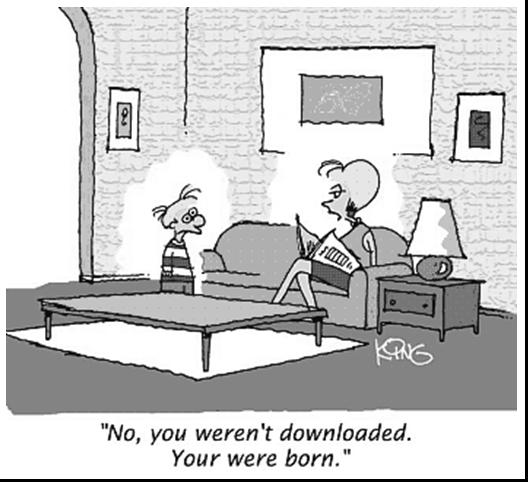
\includegraphics[width=.5\textwidth]{fig1.jpg}
\caption{A typical figure}
\label{fig:exampleFig1}
\end{figure}

In tables, try to avoid the use of colored or shaded backgrounds, and avoid
thick, doubled, or unnecessary framing lines. When reporting empirical data,
do not use more decimal digits than warranted by their precision and
reproducibility. Table caption must be placed before the table (see Table 1)
and the font used must also be Helvetica, 10 point, boldface, with 6 points of
space before and after each caption.

\bibliographystyle{sbc}
\bibliography{main}

\end{document}
